\subsection{Расширенные контекстно-свободные грамматики}

На практике оказывается удобно пользоваться расширенной контекстно-свободной или EBNF грамматикой. То-есть такой грамматикой, у которой в правых частях правил могут использоваться конструкции регулярных выражений. Необходимость использования EBNF в инструментах генерации анализаторов обоснована в работе~\cite{Diploma}.

Поддержка регулярных выражений в правых частях правил (EBNF-грамматики) получается естественным образом. Для этого правая часть правила представляется как конечный автомат. LR-ситуация в таком случае может быть представлена парой: правило (нетерминал+КА) и номер состояния (соответствует позиции маркера в классическом определении). Проблемы определения левой границы отрезка в магазине, соответствующего текущему правилу, в данном подходе не существует, так как стек вызовов рекурсивных функций хранит информацию о начале анализа по правилу.

В качестве примера рассмотрим грамматику арифметических выражений без приоритетов :

\hspace{0,9cm} 1) $E \rightarrow E $'$+$'$ E$

\hspace{0,9cm} 2) $E \rightarrow E $'$*$'$ E$

\hspace{0,9cm} 3) $E \rightarrow $'$($'$E$'$)$'

\hspace{0,9cm} 4) $E \rightarrow $'$a$' 

Так-как будет необходимо строить LR-автомат, то пополним грамматику. Добавим стартовый нетерминал и ещё одно правило.

\hspace{0,9cm} 1) $S \rightarrow E$

Грамматика примет вид:

\hspace{0,9cm} 1) $S \rightarrow E$

\hspace{0,9cm} 1) $E \rightarrow E $'$+$'$ E$

\hspace{0,9cm} 2) $E \rightarrow E $'$*$'$ E$

\hspace{0,9cm} 3) $E \rightarrow $'$($'$E$'$)$'

\hspace{0,9cm} 4) $E \rightarrow $'$a$' 


В данном случае удобно объединить правила 1) и 2) в одно:

\hspace{0,9cm} $E \rightarrow E ($'$+$' | '$*$'$) E$
 
Далее:
  
\hspace{0,9cm} $E \rightarrow (E ($'$+$' | '$*$'$) E) | ($ '$($'$E$'$)$' $) | $'$a$'                                      (1).

Используя конструкции EBNF мы смогли уменьшить количество правил в грамматике  до двух:

\hspace{0,9cm} $E \rightarrow E ($'$+$' | '$*$'$) E$
  
\hspace{0,9cm} $E \rightarrow (E ($'$+$' | '$*$'$) E) | ($ '$($'$E$'$)$' $) | $'$a$'


\subsubsection{Построение ДКА}

Для того, чтобы построить табличный LR анализатор необходимо преобразовать расширенную  контекстно-свободную грамматику. Нужно избавиться от конструкции BNF в правых частях. Однако можно попробовать обойтись без преобразований грамматики.

Существуют способы поддержки расширенной контекстно-свободной грамматики на уровне анализатора, без преобразований входной грамматики. Для этого нужно переопределить функцию goto. Можно заменить позицию точки в правиле на номер состояния конечного автомата, построенного по соответствующему регулярному выражению. Заметим, что определённая выше функция goto может быть описана в терминах конечного автомата. В этом случае регулярное выражение и, следовательно, построенный по нему автомат очень прост.  

Для построения конечного автомата по регулярному выражению воспользуемся алгоритмом Томпсона~\cite{DrgBook}. Результатом работы данного алгоритма является недетерминированный конечный автомат. Так как правая часть правила (1) - регулярное выражение, то применим к ней алгоритм Томпсона.% Получим следующий НКА: **здесь должен быть граф**

Каждое состояние и каждый переход КА должны преобразоваться в состояние и переход LR автомата соответственно. Заметим, что в в полученном НКА много $\varepsilon$-переходов. Например, каждая альтернатива вносит два дополнительных состояния и 4 $\varepsilon$-перехода. Чтобы уменьшить количество переходов в результирующем LR-автомате можно преобразовать НКА в детерминированный конечный автомат(ДКА). Для этого применим стандартный алгоритм преобразования НКА в ДКА~\cite{DrgBook}. %Полученный в результате преобразований ДКА будет выглядеть следующим образом:**здесь должен быть граф**

На практике удобно представить результирующий ДКА в виде тройки (S,F,R), где S -- начальное состояние ДКА , F -- множество конечных состояний и R -- множество функций перехода (правил), задающее ДКА.

\subsubsection{Построение множества ситуаций}

Перейдём к построению LR-ситуаций. Как было сказано выше, основная идея состоит в том, что точку из классического определения ситуации нужно заменить состоянием ДКА, построенного по правой части правила, как описано выше. Поясним. Предположим, что правило грамматики не содержит конструкций BNF. Например:

\hspace{0,9cm} $E \rightarrow E $'$+$'$ E$

Множество ситуаций для данного правила:

\hspace{0,9cm} 1) $E \rightarrow .E $'$+$'$ E$

\hspace{0,9cm} 2) $E \rightarrow E. $'$+$'$ E$

\hspace{0,9cm} 3) $E \rightarrow E $'$+$'$ .E$

\hspace{0,9cm} 4) $E \rightarrow E $'$+$'$ E.$

Теперь построим ДКА в соответствии с нашим алгоритмом. 
%\begin{figure}[h]
%	\centering
%		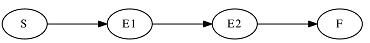
\includegraphics[width=8cm,height=1.5cm]{Simple.jpeg}
%	\label{fig:Simple}
%	\caption{}
%\end{figure}

У построенного ДКА четыре состояния: $S_{1}$ , $S_{2}$ , $S_{3}$ , $S_{4}$. Сопоставим состоянию $S_{1}$ ситуацию $E \rightarrow .E $'$+$'$ E$, $S_{2}$ ситуацию $E \rightarrow E $'$.+$'$ E$ и так далее. В итоге получим соответствие: 

\hspace{0,9cm} $S_{1}$ - $E \rightarrow .E $'$+$'$ E$

\hspace{0,9cm} $S_{2}$ - $E \rightarrow E .$'$+$'$ E$

\hspace{0,9cm} $S_{3}$ - $E \rightarrow E $'$+$'$ .E$

\hspace{0,9cm} $S_{4}$ - $E \rightarrow E $'$+$'$ E.$

Таким образом, каждой LR-ситуации мы смогли сопоставить состояние ДКА, построенного по правой части правила. Заметим, что ситуация характеризуется правилом, для которого она строится и положением точки в правой части этого правила. Теперь вернёмся к предыдущему примеру и обобщим ситуацию. 

В правой части правила - регулярное выражение. Выше мы построили по нему ДКА. Теперь построим для каждого состояния ДКА LR-ситуацию. 

Для этого сперва опишем структуру данных, в которой будем сохранять одну ситуацию. Ситуация строится для правила грамматики. Правило -- это нетерминал в левой части и ДКА, построенный по правой части. ДКА задаётся стартовым состоянием, множеством правил перехода и множеством конечных состояний. Правило перехода для ДКА -- номер текущего состояния, принимаемый символ, номер состояния, в которое переходит ДКА, приняв данный символ. Всю эту информацию необходимо хранить, для дальнейшей работы с ней. В итоге для этого потребуется структура со следующими полями:

\begin{itemize}
\item Номер правила.
\item Левая часть правила(нетерминал).
\item Номер текущего состояния ДКА.
\item Символ принимаемый ДКА в данном состоянии.  
\item Номер состояния ДКА, в которое он перейдёт приняв данный символ.
\item Номер начального состояния ДКА.
\item Номера конечных состояний ДКА.
\end{itemize}

Заметим, что эта информация состоит из двух частей: информации о ДКА в целом и правило перехода. Это ляжет в основу функции построения множества ситуаций по ДКА.

 \begin{verbatim} 
  create_items (DFA | 
 (DFA построен для правила с номером = prd_num
      и нетерминалом в левой части = prd_name )
  && (DFA = s,f,{rule | rule = (cur_num,symb,next_num)})) =
 {(prod_number,prod_name,item_number,symbol,
   next_number,start_state,finale_state)|
   prod_number = prd_num, prod_name = prd_name,
   item_number = cur_num,symbol = symb, 
   next_number = next_num,start_state = s, finale_state = f}
\end{verbatim}


\subsubsection{Вычисление GOTO}

Вычисление функции GOTO -- очень дорогая операция. При анализе вызов происходит при каждом вызове функции parse. По этому вычисление GOTO каждый раз сильно ухудшит производительность. Самое простое решение этой проблемы -- вычислить значения функции заранее, на стадии генерации данных.

На данном этапе проще всего вычислить GOTO для всех возможных пар (состояние, символ) и сконструировать коллекцию, в которой , вместо вычислений, будет производиться поиск при анализе. В качестве ключей можно взять, например, значение hash-функции от значения параметров, для которых вычислено соответствующее значение.

Основа алгоритма - стандартный алгоритм вычисления GOTO при LR анализе, подробное описание которого можно найти в ~ \cite{DrgBook}. Небольшое изменение лишь в том, что ситуация имеет специальный вид.








